
\subsubsection{AIL Feeders}

\begin{frame}[fragile]
    \frametitle{AIL feeders Importers}
    \begin{itemize}
        \item {\bf 12+ feeders are available} for all AIL users to feed from external sources
        \item External feeders can run anywhere and are completely separated from AIL framework
        \item The feeder can use their {\bf own internal logic} and even push JSON metadata
        \item Feeder are then pushing the generated JSON to AIL API
    \end{itemize}
\end{frame}

% \begin{frame}[fragile]
%    \frametitle{Feeding AIL with Twitter posts and associated urls}
%         \begin{itemize}
%                 \item AIL - feeder from Twitter\footnote{\url{https://github.com/ail-project/ail-feeder-twitter}}
%                 \item The AIL-feeder-twitter {\bf search specific keywords on Twitter} using Twint (without API), crawls the urls and pushes the results in AIL
%                 \item The JSON format format can be extended via meta fields
%         \end{itemize}
% \end{frame}

\begin{frame}[fragile]
   \frametitle{Certificate transparency feeder for AIL}
    \begin{itemize}
        \item ail-feeder-cti\footnote{\url{https://github.com/ail-project/ail-feeder-ct}} is a generic software to extract information from a certstream server (certificate transparency)
        \item All metadata extracted will be processed by AIL
        \item Onion addresses crawled automatically by AIL if seen in a certificate 
    \end{itemize}
\end{frame}

\begin{frame}[fragile]
    \frametitle{GitHub archive and GitHub repository}
    \begin{itemize}
        \item ail-feeder-gharchive\footnote{\url{https://github.com/ail-project/ail-feeder-gharchive}} is a generic software to extract informations from {\bf GHArchive}, collect and feed AIL via AIL ReST API
        \item ail-feeder-github-repo\footnote{\url{https://github.com/ail-project/ail-feeder-github-repo}} is collecting from a GitHub repository and push everything to AIL
        \item For monitoring a set of {\bf suspicious git repositories} or finding leaks on existing or managed git repositories, it's a simple way to feed AIL with such source.
    \end{itemize}
\end{frame}

\begin{frame}[fragile]
    \frametitle{AIL LeakFeeder}
    \begin{itemize}
        \item ail-feeder-leak\footnote{\url{https://github.com/ail-project/ail-feeder-leak}} automates the process to feed leaked large files automatically to AIL
    \end{itemize}
    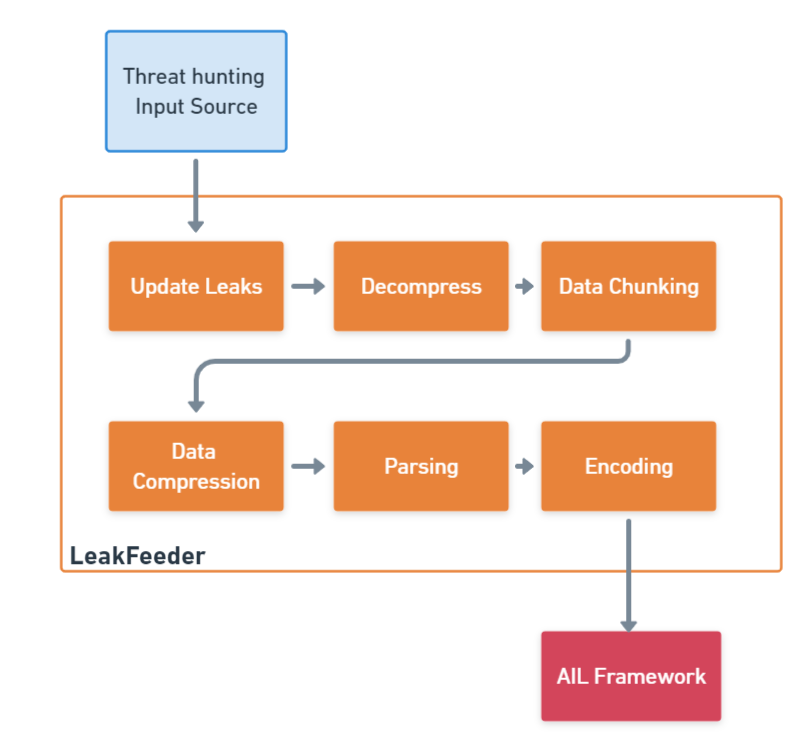
\includegraphics[scale=0.20]{./images/feeder_leak.png}
\end{frame}

\begin{frame}[fragile]
    \frametitle{AIL feeder ActivityPub}
    \begin{itemize}
        \item ail-feeder-activity-pub\footnote{\url{https://github.com/ail-project/ail-feeder-activity-pub}} is feeder for the ActivityPub standard used in distributed social networks (e.g. Mastodon)
        \item Accounts are required on the ActivityPub instance to get the stream
    \end{itemize}
\end{frame}

\begin{frame}[fragile]
    \frametitle{AIL feeder telegram}
    \begin{itemize}
        \item ail-feeder-telegram\footnote{\url{https://github.com/ail-project/ail-feeder-telegram}} is a {\bf Telegram feeder}
        \item An API ID/hash for Telegram is required and linked to your Telegram phone number
    \end{itemize}
\end{frame}

\begin{frame}[fragile]
    \frametitle{More feeders}
    \begin{itemize}
        \item ail-feeder-discord\footnote{\url{https://github.com/ail-project/ail-feeder-discord}} is a generic {\bf Discord} feeder for AIL
        \item ail-feeder-atom-rss\footnote{\url{https://github.com/ail-project/ail-feeder-atom-rss}} is an {\bf Atom and RSS reader} and feeder for AIL   
        \item ail-feeder-jsonlogs\footnote{\url{https://github.com/ail-project/ail-feeder-jsonlogs}} is a {\bf JSON aggregator} to submit generic JSON input into AIL
    \end{itemize}
\end{frame}

